\section{A Case Study}
\label{sec:case-study}

%\begin{figure}[htb]
%\begin{tikzpicture}
%	\node[draw] (drive0) at (0,0) {$drive_0$};
%	\node[draw] (drive1) at (2,0) {$drive_1$};
%	\node (driveDots) at (4,0) {$\dots$};
%	\node[draw] (driveN) at (6,0) {$drive_n$};
%
%	\draw (drive0) -- (0,-1);
%	\draw (drive1) -- (2,-1);
%	\draw[dashed] (driveDots) -- (4,-1);
%	\draw (driveN) -- (6,-1);
%	\draw (0,-1) -- (6,-1);
%
%	\draw (3,-1) -- (3,-2);
%
%	\node[draw] (changer0) at (0,-3) {$changer_0$};
%	\node[draw] (changer1) at (2.5,-3) {$changer_1$};
%	\node (changerDots) at (4.2,-3) {$\dots$};
%	\node[draw] (changerN) at (6,-3) {$changer_n$};
%
%	\draw (changer0) -- (0,-2);
%	\draw (changer1) -- (2.5,-2);
%	\draw[dashed] (changerDots) -- (4.2,-2);
%	\draw (changerN) -- (6,-2);
%
%	\draw (0,-2) -- (6,-2);
%
%	\node[draw] (client0) at (10,0) {$client_0$};
%	\node[draw] (client1) at (10,-1) {$client_1$};
%	\node (clientDots) at (10,-2) {$\dots$};
%	\node[draw] (clientN) at (10,-3) {$client_n$};
%
%	\draw (client0) -- (8,0);
%	\draw (client1) -- (8,-1);
%	\draw[dashed] (clientDots) -- (8,-2);
%	\draw (clientN) -- (8,-3);
%
%	\draw (8,0) -- (8,-3);
%\end{tikzpicture}
%\caption{Overview of the tape library architecture.}
%\label{easy}
%\end{figure}

To illustrate an ISI architecture, this section will describe a tape library
simulation. This example does not use any library support (except the Go
standard library) and serves to show how a large-scale tape system can be
simulated in a highly concurrent environment in a relatively simple manner.

A large-scale tape system (or \emph{library}) consists of a number of tape
drives and one or more robots (or \emph{changers}). Our example simulates
low-level client access to the library by instructing the changer to mount a
tape in a drive and, when ready, issue I/O requests directly to the drive.
While this is obviously a simple example, it does, however, reflect how clients
interact with a tape library in a \emph{real-world} manner.

The example is also meant to highlight the instinctive implementation. The
system includes three types of processes: changers, drives and clients. They
are implemented to behave as the real-world process that they model. This means
that they wait when they would in the real world and the code generally flows
as one would implement an actual library controller.

An important and distinctive feature of ISI is that mutual exclusion is
implicitly ensured. For instance, a drive must only be allocated to and used by
\emph{one} client at a time. This sequentiality is trivially provided due to
the sequential nature of the processes. This, of course, is not a feature
unique to ISI, but for any communicating process architecture. For any
process-based architectures this is a benefit resulting from explicitly
disallowing any sharing of data; a so-called
\emph{share-nothing} architecture.



Listing~\ref{basic-types} shows the basic types that are used in the
simulation\footnote{Full source code available at
\url{http://github.com/kbj/papers/cpa15/src}}. All requests carry a command
(\verb|mount|,
\verb|unmount|, \verb|read|, etc.), as well as a \verb|response|
channel to reply on. Similarly, the \verb|response| contains the duration
of the operation, as well as an optional \verb|request| channel. The
purpose of this channel is to	enable one-to-one communication between two
processes explicitly.

\begin{lstlisting}[caption={Basic types for tape simulation}, label=basic-types]
type request struct {
    cmd   command
    ch    chan response
    clock time.Time
}

type response struct {
    t     time.Duration
    ch    chan request
    clock time.Time
}

type library struct {
    changers chan request
    drives   chan request
}
\end{lstlisting}

Here, the library basically consists of two any-to-any channels. Changers and
drives receive messages on those two channels respectively, but never write to
them. Messages sent on Go channels do not carry a destination, so replies would
not end up with the original sender if written to the channel.


The code in these listings uses \emph{rendezvous-style} communication channels
as in CSP. Go has support for asynchronous messaging (through buffered
channels) and the performance results in section~\ref{sec:results} includes
results where this has been used. Inappropriate buffering could impact the
causality constraints or correctness, because the use of buffered channels
might cause a process to think that a message has been handled even though it
still lingers in the channel buffer. To avoid this, we employ a request/reply
idiom common in the Go community where we exploit the ability to communicate
channels along the channels themselves as in the $\pi$-calculus. Being able to
pass a channel to another process is useful as it allows the process to create a
dedicated \emph{reply} channel for a single request, ensuring that no other
communication will happen until the unique response is received. The code in
listing~\ref{reqresp} shows how this can be done, and
figure~\ref{reqresp-illustration} illustrates how this is employed in our
simulation to chain multiple processes. The request and response messages
exchanged are represented by \lstinline{req} and \lstinline{resp} respectively.
In general the messages carry a payload, which for requests are the channel a
reply should be directed to. For responses the payload is a channel that can be
used for further communication, but may (as in step 6 of
figure~\ref{reqresp-illustration}) exclude this to indicate that no further
communication is expected.
%Similar techniques are outlined in\cite{dyn-proc-net-go}.


\begin{lstlisting}[caption={Request/response using Go channels},label={reqresp}]
func request(ch chan response) {
    go func() { ch <- response{} }()
}

func client() {
    ch := make(chan response)
    request(ch);    // start work in goroutine
    <-ch            // wait for completion
}
\end{lstlisting}

\begin{figure}[htb]
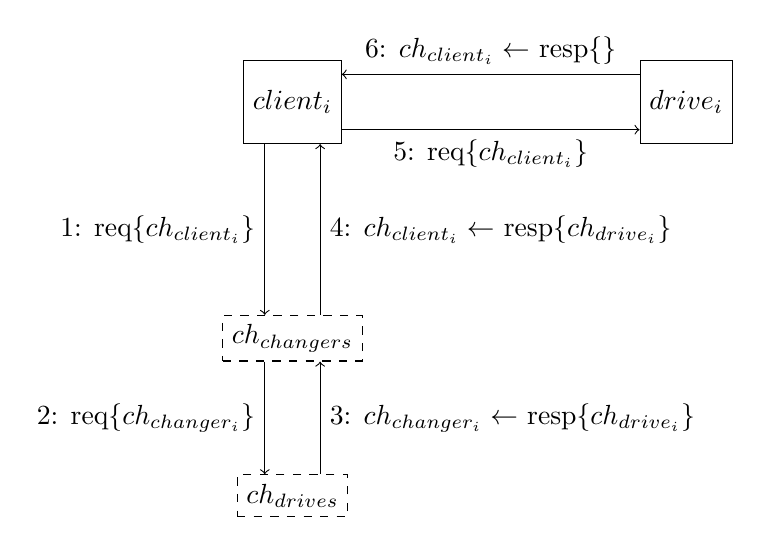
\begin{tikzpicture}
	\node[draw,minimum size=30pt] (client) at (0,1) {$client_i$};

	\node[draw,dashed] (changers) at (0,-2) {$ch_{changers}$};

	\node[draw,dashed] (drives) at (0,-4) {$ch_{drives}$};

	\draw[->] ([xshift=-10pt]client.south) -- ([xshift=-10pt]changers.north) node[left,midway] {1: req\{$ch_{client_i}$\}};

	\draw[->] ([xshift=-10pt]changers.south) -- ([xshift=-10pt]drives.north) node[left,midway] {2: req\{$ch_{changer_i}$\}};

	\draw[<-] ([xshift=10pt]changers.south) -- ([xshift=10pt]drives.north) node[right,midway] {3: $ch_{changer_i} \leftarrow$ resp\{$ch_{drive_i}$\}};

	\draw[->] ([xshift=10pt]changers.north) -- ([xshift=10pt]client.south) node[right,midway] {4: $ch_{client_i} \leftarrow$ resp\{$ch_{drive_i}$\}};

	\node[draw,minimum size=30pt] (drive) at (5,1) {$drive_i$};

	\draw[->] ([yshift=-10pt]client.east) -- ([yshift=-10pt]drive.west) node[below,midway] {5: req\{$ch_{client_i}$\}};
	\draw[<-] ([yshift=10pt]client.east) -- ([yshift=10pt]drive.west) node[above,midway] {6: $ch_{client_i} \leftarrow$ resp\{\}};
\end{tikzpicture}
\caption{Request/reply flow in ISI. The dashed boxes denotes many-to-many
channels ($ch_{changers}$ and $ch_{drives}$). Individual processes are denoted
by their type name and an index such as $drive_i$. Similarly, individual
channels are denoted by e.g. $ch_{client_i}$. The labels describe the
request flow and whether it is a request or reply. In the figure we see how a
client sends a request carrying a reply channel to the changers (1). A (one)
changer received the request and sends a new request to the drives, again
carrying its own reply channel in the request (2). A (one) drive responds to
the changer with a channel to receive further requests on (3), which the
changer simply pass on to the client (4). Finally the client initiates a fresh
request/reply with the specific drive that was allocated by the changer (5 and
6).}
\label{reqresp-illustration}
\end{figure}


Next, we define the \emph{processes}. These are simply regular looping
functions. In this system we are interested in measuring the perceived wait
time and actual I/O time the system can provide given enough requests and a
certain number of resources (changer and drives). Here, enough requests, mean
that no client will ever stop and wait in simulated time. It will immediately
issue a new request.

The key here is that time measurement thus becomes \emph{relative}. This vastly
simplifies the time keeping, and this example does not use any kind of
explicit time synchronization, besides lazily updating a world clock based on
the relative measurements.

\begin{lstlisting}[caption={Tape media changer},label=changer]
func changer(lib *library) {
    var clock time.Time
    var resp  reponse

    // channel to expect response on
    ch := make(chan response)

    for {
        req := <-lib.changers

        // update clock
        if req.clock.After(clock) { clock = req.clock }

        // unmount skipped, for brevity

        lib.drives <- request{mount, ch, clock}
        resp = <-ch
        clock = resp.clock // update clock

        req.ch <- response{clock.Sub(req.clock), resp.ch, clock}
    }
}
\end{lstlisting}


The two processes providing the majority of measurements are the changer and
the drive, shown in listing~\ref{changer} and listing~\ref{drive} respectively.
Notice that the local clock is updated after each received message.
The received clock is ensured to be in the future relative to the local clock.
If a process (client) has not issued any requests for a period time, the local
clock will have fallen behind, so the process instead replies with its
(possibly also outdated, but monotonically higher) clock to inform the client
that time has moved on. In this example, this is irrelevant to the client. It
knows precisely how long it has waited for at tape to be mounted, and how long
the actual I/O request took. These durations are calculated by the changer and
drive processes, and will thus correctly indicate a longer wait time, if no
drives are available or all changers are busy processing other requests.


\begin{lstlisting}[caption={Tape drive},label=drive]
func drive(lib *library) {
    var clock time.Time
    var req   request
    var t     time.Duration // time of operation

    // channel to expect request on
    ch := make(chan request)

    for {
        req = <-lib.drives

        // update clock
        if req.clock.After(clock) { clock = req.clock }

        switch req.cmd {
        case mount:
            // mount tape
            t = ... // time real mount, or simulate
            clock = clock.Add(t)
            req.ch <- response{t, ch, clock}

            // wait for I/O request
            req = <-ch

            // do request
            t = ... // time real I/O, or simulate
            clock = clock.Add(t)

            req.ch <- response{t, nil, clock}

        case unmount:
            // unmount skipped, for brevity
        }
    }
}
\end{lstlisting}

The client follows the same (but simpler) pattern, but is excluded for brevity.
To run these processes concurrently, we use the \lstinline{go} keyword
(listing~\ref{main}). This starts the function in a new concurrent process (or
\emph{goroutine}) and immediately returns control to the calling process. This
can be done any number of times to start multiple processes.

\begin{lstlisting}[caption={Simulation entry point},label=main]
func main() {
    go changer(lib); go changer(lib); ...
    go drive(lib); ...
    for ... { go client(lib) }
    ...
}
\end{lstlisting}

This example serves to show how a simulation in itself constitutes a measurable
design that evolves directly into a prototype. Wherever I/O requests are
simulated, the code can be swapped for actual I/O code, using the same
process-oriented architecture. To validate the system, we can run an I/O trace
through the client on simulated drives and analyse the results. The reverse is
also possible by simulating an I/O workload on real devices. This could be
valuable to operators of HPC systems, where a certain work load is anticipated
and want to get a feeling for how it would perform on their system.



\subsection{Results}
\label{sec:results}

To verify that the ISI communicating process architecture is viable, we have
simulated our library at large scale. We simulate a period of 90 days, with up
to 80,000 drives, 10,000 changers and 160,000 clients, totalling 250,000
processes. This has been done for one, two, four and eight cores using both
buffered and unbuffered channels, for at total of twelve different
configurations. Each configuration is run five times and an average is
calculated, while handling outliers. Time measurement is performed with the
\verb|time| builtin of the Bash shell, configured for wall-clock time (which is
\emph{not} the default configuration). The
simulation is done on a 16 core AMD Opteron 6272 CPU, running at 2.1GHz. This
CPU has two NUMA domains, so \verb|taskset(1)| has been used to force each
benchmark onto one domain. The node is dual socket, so there are 32 cores
available in total, sharing 128 GB of memory. Our largest simulation requires
just under 7 GB of memory, which is small enough for us to ensure that it will
be located on a single NUMA domain, minimizing data movement. Software-wise,
the node is running Ubuntu GNU/Linux 14.04.2 LTS with Go version 1.4.2,
linux/amd64. The node is part of a cluster, so the node was
allocated for exclusive use to minimize influence of other running tasks.

The results are shown in
figure~\ref{fig:runtime1}-\ref{fig:runtime-buffered}. The first four figures
shows the running time for one, two, four and eight cores respectively with
unbuffered and buffered channels. The last two compares the running time of
different number of cores for unbuffered and buffered channels respectively. A
graph comparing different number of cores for buffered channels of size 1000
has been left out due to its close similarity to
figure~\ref{fig:runtime-buffered}. The raw results are presented in
table~\ref{tab:runtime-unbuffered} and~\ref{tab:runtime-buffered}, with the
fastest runtime highlighted for each number of processes. Again, the
raw results for a channel buffer size of 1000 has been left out for
brevity. The scripts used for benchmarking as well as all raw results and
scripts needed to produce the graphs are available at
\url{http://github.com/kbj/papers/cpa15/bench}.

\begin{table}
	\caption{Runtime results in seconds (unbuffered). Fastest highlighted.}
	\label{tab:runtime-unbuffered}
	\begin{tabular}{rrrrr}
		\hline
		Processes & 1 core & 2 cores & 4 cores & 8 cores\\
		\hline
		25 & \textbf{2.14} & 4.14 & 4.04 & 4.00 \\
		100 & 9.22 & \textbf{4.96} & 5.82 & 6.15 \\
		250 & 23.90 & 10.77 & \textbf{10.71} & 13.39 \\
		1000 & 101.09 & 37.75 & \textbf{32.00} & 37.77 \\
		2500 & 245.64 & 80.37 & \textbf{70.10} & 75.45 \\
		10000 & 292.40 & 365.42 & 585.33 & \textbf{243.83} \\
		25000 & \textbf{397.34} & 419.40 & 652.45 & 528.45 \\
		100000 & 881.00 & \textbf{726.77} & 902.13 & 1788.21 \\
		250000 & 1839.43 & \textbf{1307.85} & 1392.19 & 3671.10 \\
		\hline
	\end{tabular}
\end{table}

\begin{table}
	\caption{Runtime results in seconds (buffered, size 100). Fastest highlighted.}
	\label{tab:runtime-buffered}
	\begin{tabular}{rrrrr}
		\hline
		Processes & 1 core & 2 cores & 4 cores & 8 cores\\
		\hline
		25 & 2.22 & \textbf{2.11} & 2.96 & 2.91 \\
		100 & 5.11 & 4.96 & \textbf{4.44} & 4.58 \\
		250 & 27.09 & 12.63 & \textbf{9.86} & 10.78 \\
		1000 & 110.72 & 43.19 & \textbf{32.16} & 33.19 \\
		2500 & 110.83 & 122.83 & 76.30 & \textbf{72.19} \\
		10000 & 123.91 & \textbf{121.59} & 174.01 & 315.17 \\
		25000 & 136.47 & \textbf{123.72} & 176.50 & 322.98 \\
		100000 & 153.77 & \textbf{136.59} & 184.69 & 309.25 \\
		250000 & 691.15 & \textbf{139.34} & 191.30 & 311.50 \\
		\hline
	\end{tabular}
\end{table}


\begin{figure}
	\centering
	\includegraphics[width=\textwidth]{plots/1-core.pdf}
	\caption{Runtime of a large scale tape library simulation (1 core)}
	\label{fig:runtime1}
\end{figure}

\begin{figure}
	\centering
	\includegraphics[width=\textwidth]{plots/2-cores.pdf}
	\caption{Runtime of a large scale tape library simulation (2 cores)}
	\label{fig:runtime2}
\end{figure}

\begin{figure}
	\centering
	\includegraphics[width=\textwidth]{plots/3-cores.pdf}
	\caption{Runtime of a large scale tape library simulation (4 cores)}
	\label{fig:runtime4}
\end{figure}

\begin{figure}
	\centering
	\includegraphics[width=\textwidth]{plots/4-cores.pdf}
	\caption{Runtime of a large scale tape library simulation (8 cores)}
	\label{fig:runtime8}
\end{figure}

\begin{figure}
	\centering
	\includegraphics[width=\textwidth]{plots/unbuffered.pdf}
	\caption{Runtime of a large scale tape library simulation (unbuffered channels)}
	\label{fig:runtime-unbuffered}
\end{figure}

\begin{figure}
	\centering
	\includegraphics[width=\textwidth]{plots/buffered-100.pdf}
	\caption{Runtime of a large scale tape library simulation (buffered channels, size 100)}
	\label{fig:runtime-buffered}
\end{figure}



The first thing we observe is that using unbuffered channels with more than one
core generally performs well until the number of processes becomes unwieldy
(figure~\ref{fig:runtime-unbuffered}). This happens somewhere close to 10,000
 processes and the runtime explodes when using unbuffered channels.
The worst result is 250,000 processes running on eight cores with unbuffered
channels and is almost twelve times slower than with buffered channels. This is
not surprising as there will be high contention on the many-to-many
\verb|changers| and \verb|drives| channels.

Using buffered channels, a high process count and multiple cores, Go really
shows off its abilities (figure~\ref{fig:runtime-buffered}). The runtime is almost
unchanged going from 10,000 to 250,000 processes. This is, intuitively, an
unexpected result, but knowing that context switches between goroutines are
extremely cheap, this hints at the fact that a large fraction of the overall
runtime is due to waiting; a fraction that becomes smaller as we increase the
process count, but which does not change the runtime significantly.

Interestingly, running 250,000 processes on two cores is almost two times faster
than running on eight (table~\ref{tab:runtime-buffered} and figure~\ref{fig:runtime-buffered}). The AMD Opteron
6272 is an \emph{Interlagos}-family CPU, which is a multi-chip module
consisting of multiple dies, each with multiple dual-core \emph{Bulldozer}
modules\cite{amd-interlagos}. Realizing that our
simulation is extremely memory heavy, the results makes sense; the individual
dual-core modules can simply communicate faster, provided the two kernel
threads are scheduled on the same module.

Increasing the channel buffer size from 100 to 1,000 has almost no impact, but
still yields slower results (figures~\ref{fig:runtime1}-\ref{fig:runtime8}).
Again, this tells us that our achievable performance is bound by
our use of memory. This is not surprising, but it does pose some questions
about how to schedule goroutines for cache/core locality. While we have not
looked into this yet, Go does support goroutine \emph{pinning}, where a
goroutine can be bound to a kernel thread, which can then be pinned to a core
by using the appropriate tools provided by the operating system.
